\documentclass[12pt]{article}
\usepackage[paper=a4paper,left=30mm,right=30mm,top=35mm,bottom =35mm]{geometry}
\usepackage[utf8]{inputenc}
\usepackage[T1]{fontenc}
\usepackage{stmaryrd}
\usepackage{setspace}
\usepackage{mathrsfs}
\usepackage[ngerman]{babel}
\usepackage{amssymb}
\usepackage{amsmath}
\usepackage{fancyhdr}
\usepackage[dvips,unicode,colorlinks,linkcolor=black]{hyperref} 
\usepackage{graphicx}
\usepackage{float}

\pagestyle{fancy}
\lfoot{}
\rfoot{Paul Kremser, Tobias Grussenmeyer}
\cfoot{\thepage}
\fancyhead[L]{FPII Versuch: Mösbauereffekt}
\renewcommand{\headrulewidth}{0.6pt}
\renewcommand{\footrulewidth}{0.6pt}
\setlength{\headheight}{30pt}
\setlength{\parindent}{0pt}
% Für die Wahl der Schriftart
\newcommand{\changefont}[3]{
\fontfamily{#1} \fontseries{#2} \fontshape{#3} \selectfont}
%\renewcommand{\vec}[1]{\mathbf{#1}}
\renewcommand*\vec[1]{{\mbox{\boldmath\ensuremath{#1}}}}

\begin{document}
% keine Hurenkinder und Schusterjungen
\clubpenalty = 10000
\widowpenalty = 10000 
\displaywidowpenalty = 10000

\onehalfspacing
% Schriftart
\changefont{ptm}{m}{n} 

\begin{titlepage}
\author{Paul Kremser, Tobias Grussenmeyer}
\title{Versuch: Mösbauereffekt}
\date{Versuchsdurchführung: 1. bis 12. März 2010} 
\maketitle
\thispagestyle{empty}
\end{titlepage}


\tableofcontents
\thispagestyle{empty}
\newpage
\pagenumbering{arabic}
\section{Überblick}
Bei dem Mössbauereffekt handelt es sich um rückstoßfreie Resonanzabsorption im Gammastrahlenbereich.
Sein Namensgeber Rudolf Mössbauer erhielt für die Entdeckung 1961 den Nobelpreis. Zum besseren Verständnis des
eigentlichen Phänomens wird nun zunächst etwas Vorwissen erläutert.
\textbf{Radioaktive Strahlung:}
Im allgemeinen unterscheidet man drei Arten von Strahlung:
\textit{Die Alphastrahlung}, 
hierbei handelt es sich um Heliumskerne.
\textit{Die Betastrahlung},
hierbei handelt es sich um Elektronen.
\textit{Die Gammastrahlung},hierbei handelt es sich um hoch energetische elektromagnetische Strahlung.
Besonders gefährlich wird sie dadurch das sie nur sehr schwer abzuschirmen ist. Man benötigt ein sehr dichtes Material in der Praxis
wird meist Blei verwendet. Zusätzlich ist eine sehr dicke Matrialschicht für vonnöten um die Strahlung abzuschwächen.
\newline
\textbf{Der Mössbauereffekt},
im Rahmen seiner Dissertationsarbeit wollte Mössbauer die Wahrscheinlichkeit für die Emissionen und anschließende Absorption eines Gammaquant untersuchen.
Er ging davon aus, dass sich zwei Quanten die auf diese Weise Wechselwirken mit der doppelten Rückstoßgeschwindigkeit aufeinander zu bewegen müssten.
Diese Theorie folgt direkt aus der Impulserhaltung und schien zunächst auch durch das Experiment bestätigt zu werden. Zuerst untersuchte Mössbauer nämlich die
Resonanzabsorption bei Zimmertemperatur und darüber. Als er aber begann Quelle und Absorber abzukühlen, stieg die Intensität des Messsignals plötzlich steil an,
und zwar über die bei hohen Temperaturen gemessenen. Dies zunächst verblüffende Ergebniss konnte von Mössbauer durch die höhere Trägheit der im Festkörper
gebundenen Atome erklähren. Diese sorgt dafür das bei der Impulsbilanz der Stösse nicht mehr die Masse eines Atoms sondern die eines ganzen Mols Stoffmasse 
relevant ist. Dadurch ist der Energieübertrag sehr viel geringer und es kommt zu einer Überlappung der Linien für Absorption und Emission. Zunächst aber ein
kurzer Überblick über die Vorgänge bei Emmission und Absorbtion. 

Wenn der von uns verwendete Eisenkern von einem angeregten in einen Grundzustand übergeht, sendet er ein Gamma Quant aus. Da dieses einen von Null verschiedenen 
Impuls hat muss sich laut der Impulserhaltung auch der Impuls des Kerns geändert haben. Interpretieren wir die Bewegungsrichtung des Quants als positive
Wegrichtung so sinkt der Impuls des Kerns bei der Emission. Für das ausgesendete Quant heißt das, dass es nicht mehr exakt die Energie des Zustandsübergangs
hat da der Impulsübertrag einen Energieübertrag impliziert. Geht man von freiem Eisenkern aus wie auch Mössbauer es zunächst tat so ist diese Energieübertrag
durchaus signifikant. Betrachtet man die Absorption so findet auch hier ein Energieübertrag statt, allerdings steigt hier der Impuls des Kerns und es bleibt
nicht die gesamte Energie des Quants übrig um den Kern anzuregen. Folgende Skizze soll dies nochmal veranschaulichen.
\begin{figure}
 \includegraphics[width=0.9\linewidth]{pictures/linienskizze.ps}
 \caption{Energieverschiebung von Emissions- und Absorptionslinie}
 \label{linienskizze}
\end{figure}


Bindet man die Kerne nun aber in Kristalle ein so muss der Impuls des Photons irgentwie auf den gesamten Kristall übergehen. Im glücklichten Fall entsteht
hierbei kein Phonon im Kristall und die dem Photon fehlende Energie geht mit steigender Masse des Kristalls gegen Null. Man spricht von rückstoßfreier
Resonanzabsorption, das Photon kann nun einen anderen Kern anregen.
\section{Aufgabenstellung}
\begin{enumerate}
 \item Verkabelung des Aufbaus, Einstellungen der Elektronik (Verstärker, Delay, SCA und Gate).
 \item Energieeichung des MCA mit Hilfe eines Americium Strahlers und verschiedener metallischer Floureszenzplättchen (Aufbau mit Drehscheibe)
 \item Mit dem SCA ein Fenster auf die 14,4 KeV Linie setzen.
 \item Mit Hilfe verschiedener Aluminiumplättchen sollen Untergrundmessungen bei verschiedenen Dicken gemacht werden um später auf die Dicke Null extrapolieren zu können.
 \item Aufnahme der Spektren des Einlinien- (Eisen) absorbers und des 6-Linien- (Edelstahl) absorbers.
\end{enumerate}

\section{Theoretische Grundlagen}
Wie schon im Überblick erwähnt geht es beim Mößbauereffekt um das Auftreten rückstoßfreier Kernresonanzabsorption.
Im Fall dieses Experiments wird der Mößbauereffekt an der 14,4keV-Linie von $^{57}Fe$ beobachtet. 

\subsection{Resonanzabsorption}
Geht ein Kern unter Aussendung eines Photons von einem angeregten Zustand $E_a$ in den Grundzustand $E_g$ über und regt dieses Photon
wiederum einen anderen Kern aus dem
Grundzustand $E_g$ in den selben angeregten Zustand $E_a$ an, so spricht man von Resonanzabsorption.

Ein freies ruhendes Atom bzw. ruhender Kern mit Masse $m$ erhält bei Emission eines Photons $\gamma$ aufgrund der Impulserhaltung
gerade den entgegengesetzten Impuls des ausgesendeten Photons:
\begin{align}
 \vec{p}_g = -\vec{p}_\gamma = \hbar\vec{k}
\end{align}
Für die Energie dieses Rückstoßes erhält man mit der Photonenenergie $E^2_\gamma = \vec{p}^2_\gamma c^2$:
\begin{align}
 E_R = \frac{\vec{p}_g^2}{2m} = \frac{\vec{p}^2_\gamma}{2m} = \frac{E^2_\gamma}{2mc^2}
 \label{e_r}
\end{align}
Die Energie des Übergangs $E = E_a - E_g$ teilt sich also auf die Rückstoßenergie und die Photonenenergie auf:
\begin{align}
 E = E_R + E_\gamma
\end{align}
Somit entspricht die Energie des emmitierten Photons nicht ganz der des Übergangs. Ebenso wird bei der Absorption eines Photons durch einen freien ruhenden
Kern ein Impuls auf den Kern übertragen. Insgesamt fehlt für die Resonanzabsorption bei freien ruhenden Atomen bzw Kernen also der Energiebetrag von $2E_R$.
Damit sind die Emissions- und Absorptionslinie gegeneinander Energieverschoben. (Siehe Abbildung. \ref{energieverschiebung})
\begin{figure}
 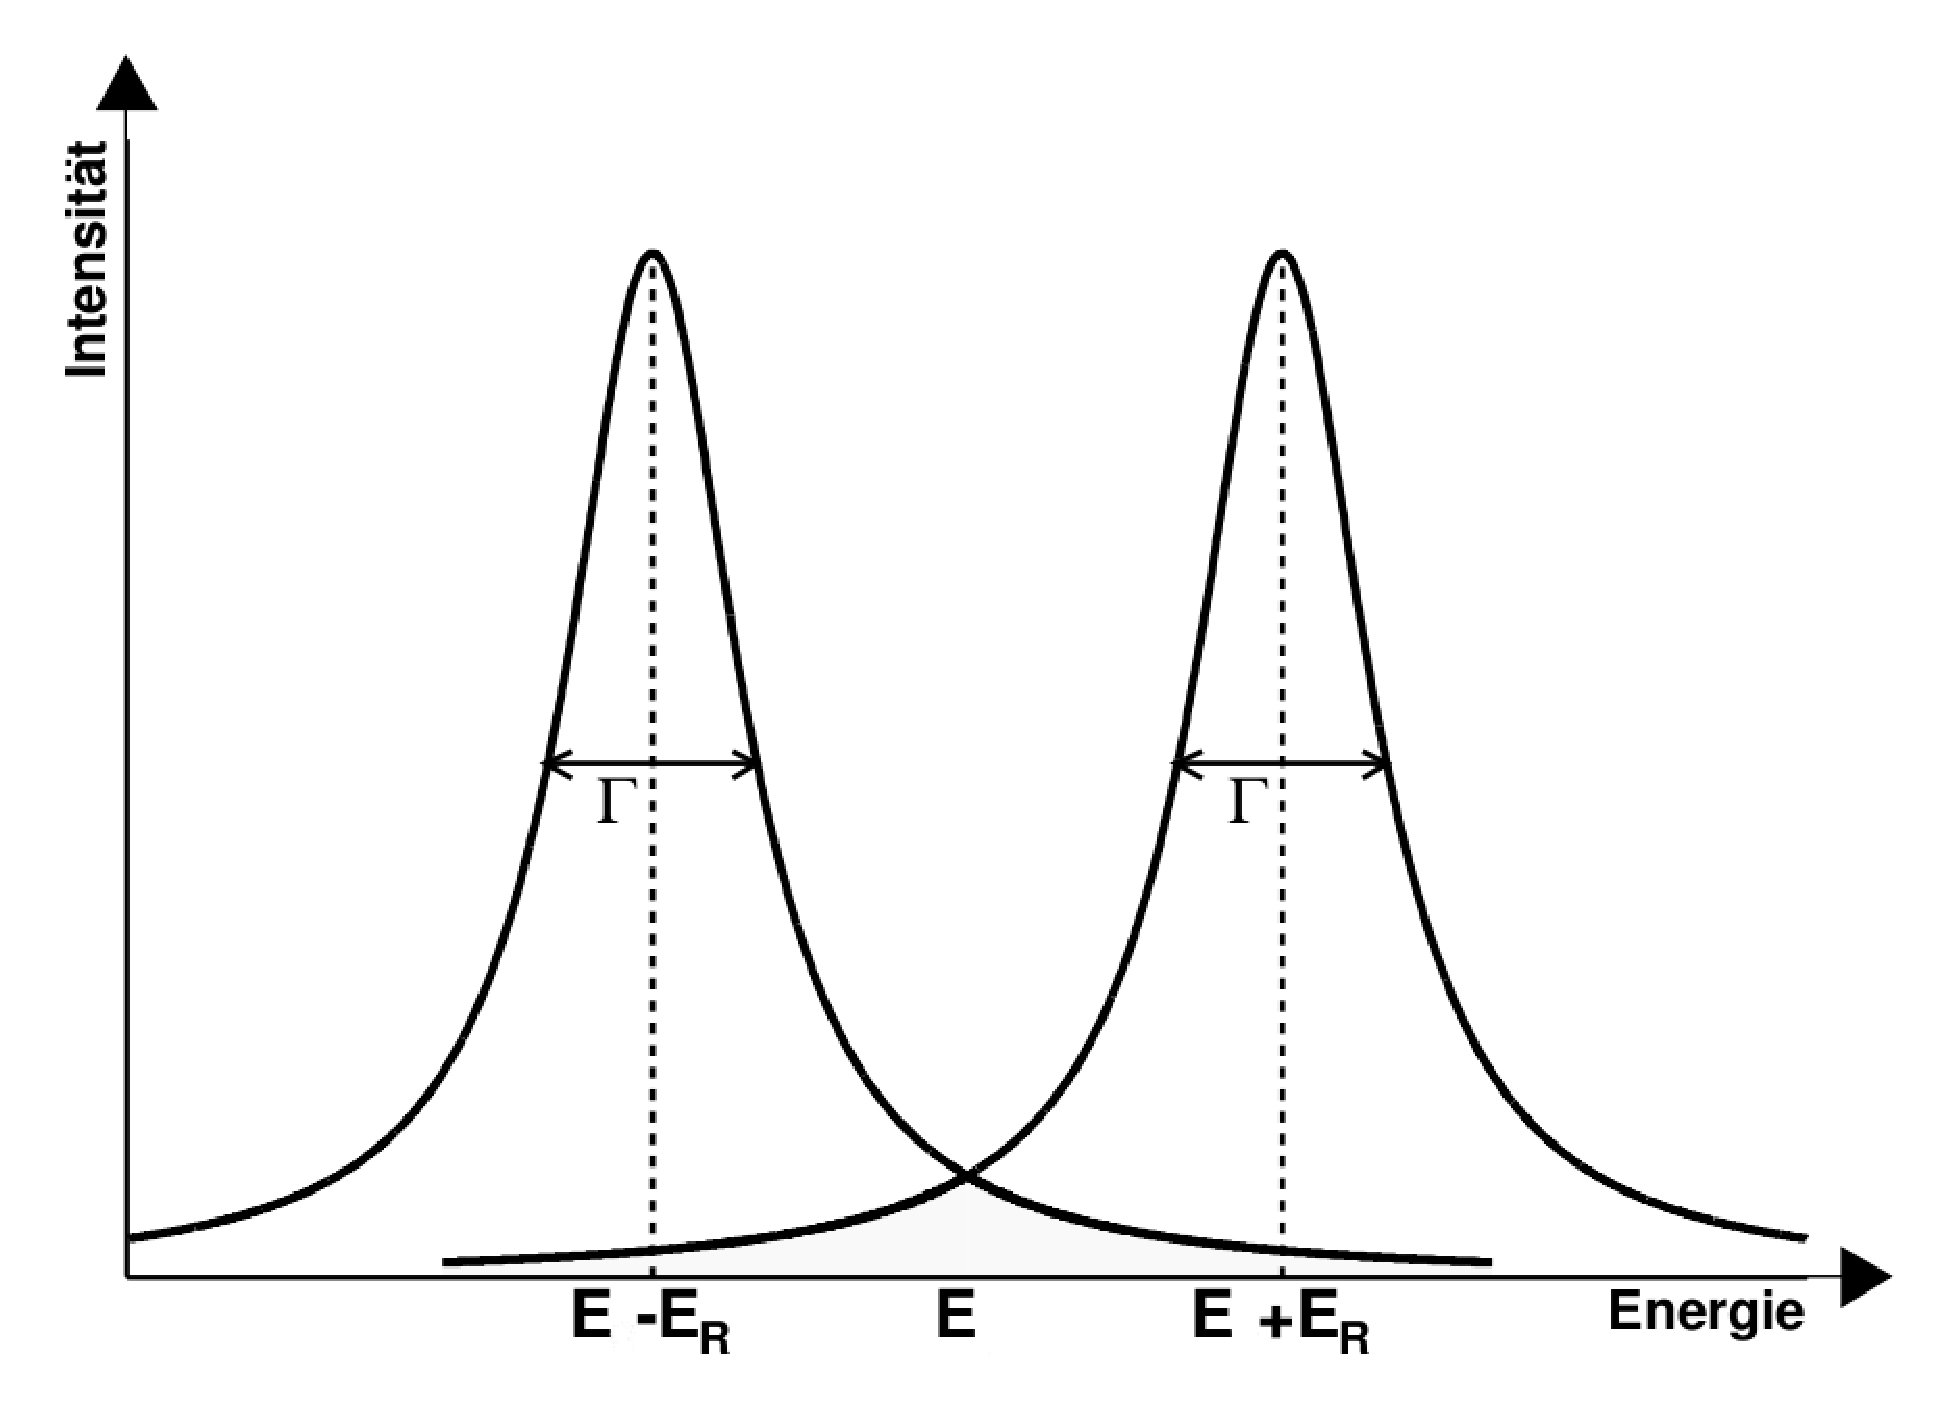
\includegraphics[width=0.9\linewidth]{pictures/energieverschiebung.eps}
 \caption{Energieverschiebung von Emissions- und Absorptionslinie}
 \label{energieverschiebung}
\end{figure}
Bei Übergängen an Atomen im Sichtbaren Bereich ist die Linienbreite, aufgrund der relativ kleinen Übergangsenergie (eV-Bereich) gegenüber der Atommasse,
groß gegenüber der Verschiebung der beiden Linien. Kommt zur natürlichen Linienbreite auch noch die Dopplerverbreiterung wenn sich die Atome ein einem Gas
befinden so kann fast vollständige Überlappung der beiden Linien erreicht werden. Es kommt also fast immer zu Resonanzabsorption.

Bei Kernübergängen im $\gamma$-Bereich ist die Übergangsenergie im keV-Bereich und somit groß gegen die Masse des Kerns. Die beiden Linien überschneiden sich
selbst mit Dopplerverbreiterung garnicht oder fast garnicht. In einem solchen System wird also keine Resonanzabsorption zu beobachten sein zumindest nicht
wenn man das System nicht dahingehend beeinflussen kann dass die Linien näher zusammenrücken. Hier kommt der Mößbauereffekt gelegen.

\subsection{Mößbauereffekt}
Rudolf Mößbauer entdeckte, dass wenn man die Kerne nicht frei vorliegen hat sondern in ein Gitter bindet, kann man erreichen das der Rückstoßimpuls $\vec{p}_g$
auf den gesamten Kristall übertragen wird. Wegen der riesigen Masse des Kristalls ist nach Gleichung \ref{e_r} damit aber, solange keine Gitterschwingungen (Phononen) angeregt werden,
fast kein Energieübertrag verbunden. Die Emissions- und Absorptionslinie sind somit nicht gegeneinander verschoben und es kann Resonanzabsorption auftreten. Die sogenannte
``rückstoßfreie Resonanzabsorption''.

\subsubsection{Debye-Waller-Faktor}
Wie schon erwähnt kann es aber auch vorkommen, dass keine rückstoßfreie Resonanzabsorption auftritt da bei der Absorption oder Emission Gitterschwingungen (Phononen) 
angeregt werden können und somit dem Photon doch wieder nicht die volle Energie des Übergangs zur Verfügung steht. Der Debye-Waller-Faktor $f$ gibt an wieviel rückstoßfreie Resonanzabsorption
auftritt. Er hängt von der Temperatur und der Übergangsenergie ab:
\begin{align}
 f = exp\left[ -\frac{3E_R}{2k_B\Theta}\left(1+\left(\frac{2T}{\Theta}\right)^2 \int\limits_{0}^{\frac{\Theta}{T}} \frac{x~dx}{e^x - 1}\right)\right]
\end{align}
und lässt sich für kleine Temperaturen $(T<<\Theta)$ und Kerne im arteigenen kubischen Gitter annähern durch:
\begin{align}
 f \approx exp \left[ -\frac{E_R}{k_B\Theta}\left(\frac{3}{2} + \left(\frac{\pi T}{\Theta}\right)^2\right)\right]
\end{align}
wobei $T$ die absolute Temperatur, $k_B$ die Boltzmannkonstante, $E_R$ die Rückstoßenergie und $\Theta$ die Debye-Temperatur ist.

\subsection{Isomerieverschiebung}
Ist die Ladungsdichteverteilung des angeregten Zustands nicht die selbe wie die des Grundzustands, wie z.B. bei dem im Versuch verwendeten $^{57}Fe$ bei dem der Kernradius
des angeregten Zustands etwas kleiner ist als der Kernradius des Grundzustands, so führt das zu unterschiedlichen Wechselwirkungsenergien des Kerns mit
der Hülle, also zu unterschiedlichen Energien der beiden Zustände. Dadurch sind das angeregte Energieniveau und das Grundnieveau um unterschiedliche Beträge gegen die
reinen Kernenergien (ohne Hüllenwechselwirkung) verschoben. Ist nun die Elektronendichte $L(0)$ am Kernort aufgrund chemischer Bindungen in Quelle und Absorber unterschiedlich,
so bewirkt das einen kleinen Unterschied in der Übergangsenergie.
\begin{align}
 E_\gamma = E_0 + \frac{2\pi}{3} L(0) \left[ R_a^2 - R_g^2\right]
\end{align}
Folglich entsteht eine kleine Verschiebung der gemessenen Linie gegenüber dem Nullpunkt der Geschwindigkeit. Diese wird als Isomerieverschiebung bezeichnet. Die Isomerieverschiebung
liegt etwa in der Größenordnung der natürlichen Linienbreite und ist ein praktisches Werkzeug zur Untersuchung von chemischen Bindungen in den verwendeten Materialien.

\subsection{Hyperfeinstrukturaufspaltung}
Die Hyperfeinstrukturaufspaltung resultiert aus der Kopplung des kernmagnetischen Moments $\mu_I$ mit dem am Kernort durch die Hüllenelektronen erzeugten Magnetfeld $B_J$.
Durch die Kopplung ist der Gesamtdrehimpus $\vec{F}$, der die Summe aus Hüllendrehimpuls $\vec{J}$ und Kernspin $\vec{I}$ ist, gequantelt:
\begin{align}
 \left|\vec{F}\right| = \hbar \sqrt{F(F+1)}
\end{align}
Die Quantenzahl $F$ nimmt in ganzzahligen Schritten die Werte von $-I$ bis $I$ an.
In unserem Fall ergibt sich somit für den angeregten Zusand $I_a = \frac{3}{2}$ eine Aufspaltung in vier Nieveaus und für den Grunzustand $I_g = \frac{1}{2}$ in zwei Nieveaus.
Mit der Auswahlregel für elektromagnetische Dipolstrahlung $\Delta m_I = 0, \pm 1$ erhält man $6$ erlaubte Übergänge. Über die Wechselwirkungsenergie
\begin{align}
 E_{mag} = \frac{\mu_I m_I}{I} B
\end{align}
lassen sich deren Energien berechnen zu:
\begin{align}
 E_\gamma = E_0 + E_{iso} - \left(\frac{\mu_a m_a}{I_a} - \frac{\mu_g m_g}{I_g} \right) B
\label{hfs}
\end{align}
\begin{figure}[H]
 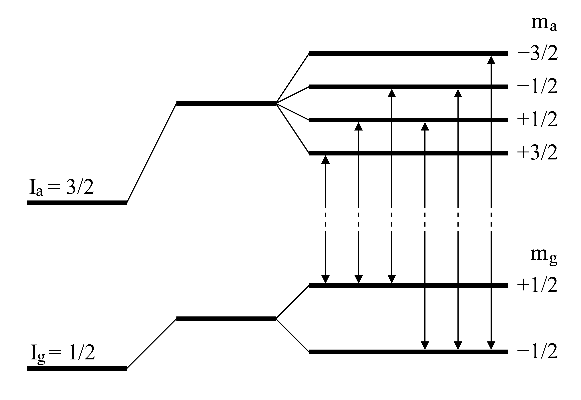
\includegraphics[width=0.9\linewidth]{pictures/termshema_eisen.eps}
 \caption{Gaußfit an 14,4keV Linie von Eisen}
\label{eisen_term}
\end{figure}
Dementsprechend erhalten wir 6 Absorptionslinien in der Transmissionskurve.
\subsection{Linienverbreiterung}
Als Linienverbreiterung bezeichnet man im allgemeinen die 
Ein Ziel des Mößbauerexperimets ist die Ausmessung des sehr schmalen Linienprofils. Aus der Halbwertsbreite der gemessenen Linie lässt sich dann die natürliche Linienbreite bestimmen.

Wegen der Heisenbergschen Unschärferelation für Energie $E$ und Zeit $t$:
\begin{align}
 \Delta E \Delta t \geq \hbar
\end{align}
verursacht die endliche Lebensdauer angeregter Zustände eine natürliche Linienbreite

Durch das Abfahren der Emissionslinie mit der Absorptionslinie durch die Variation der Geschwindigkeit ist das gemessene Linienprofil eine Faltung der lorentzförmigen
Emissions- und Absorptionskurve. Bei Verwendung von dünnen Quellen und Absorbern ist die gemessene Linie wieder eine Lorentzkurve und man erhält für den Zusammenhang
zwischen gemessener und natürlicher Linienbreite den Zusammenhang:
\begin{align}
 \label{linienbreite}
 \Gamma_{mes} = 2\Gamma
\end{align}

Im Experiment verwendet man in der Praxis jedoch meistens dicke Absorber, was leider diesen einfachen Zusammenhang zerstört. Die Dicke von Quelle und Absorber bewirkt
eine zusätzliche Verbreiterung der gemessenen Linie und lässt diese nicht mehr die Form einer Lorentzkurve haben. Nur durch umfangreiche numerische Berechnungen
lässt sich die Verbreiterung der Linie mit der effektiven Quellen- und Absorberdicke in Beziehung setzen. Die Diagramme dazu sind in Frauenfelder ??Bibtex?? zu finden.
Macht man die Annahme einer nicht resonant absorbierenden Quelle, also einer Quelle mit einer effektiven Quellendicke von 0, so muss nur die effektive Absorberdicke bestimmt
werden. Diese ist definiert durch:
\begin{align}
 T_a = f_a \beta n \sigma_0 d
\end{align}
wobei $f_a$ der Debye-Waller-Faktor des Absorbers, $\beta$ die Isotopenhäufigkeit des absorbierenden Kerns $(^{57}Fe)$ im Absorber, $n$ die atomare Dichte
des Absorbermaterials (Eisen), $\sigma_0$ der maximale Wirkungsquerschnitt und $d$ die Absorberdicke ist. Anhand dieser Größe kann dann aus einem Diagramm in Frauenfelder ??Bibtex??
die relative Verbreiterung $W = \frac{\Gamma_{mes}}{\Gamma}$ und damit die natürliche Linienbreite $\Gamma = \frac{\Gamma_{mes}}{W}$ abgelesen werden.
Eine andere Möglichkeit besteht darin statt einer Lorentzkurve auch eine Faltung aus Lorentz- und Gaußkurve an die Messwerte zu fitten. Hier repräsentiert der Gaußanteil
die Verbreiterung der Linie durch Absorber- und Quellendicke. Hier gilt dann wieder für die Halbwertsbreite des Lorenzanteils der Zusammenhang aus Gleichung \ref{linienbreite}.
Somit lässt sich auch die natürliche Linienbreite mit $\Gamma = \frac{\Gamma_{mes}}{2}$ wieder leicht daraus bestimmen.
\section{Versuchsaufbau}

Mössbauer selbst untersuchte in seinem Versuchsaufbau die Emission des Absorbers hinter einer Abschirmung. Folgende Skizze soll seinen Versuchsaufbau veranschaulichen.

\begin{figure}[H]
 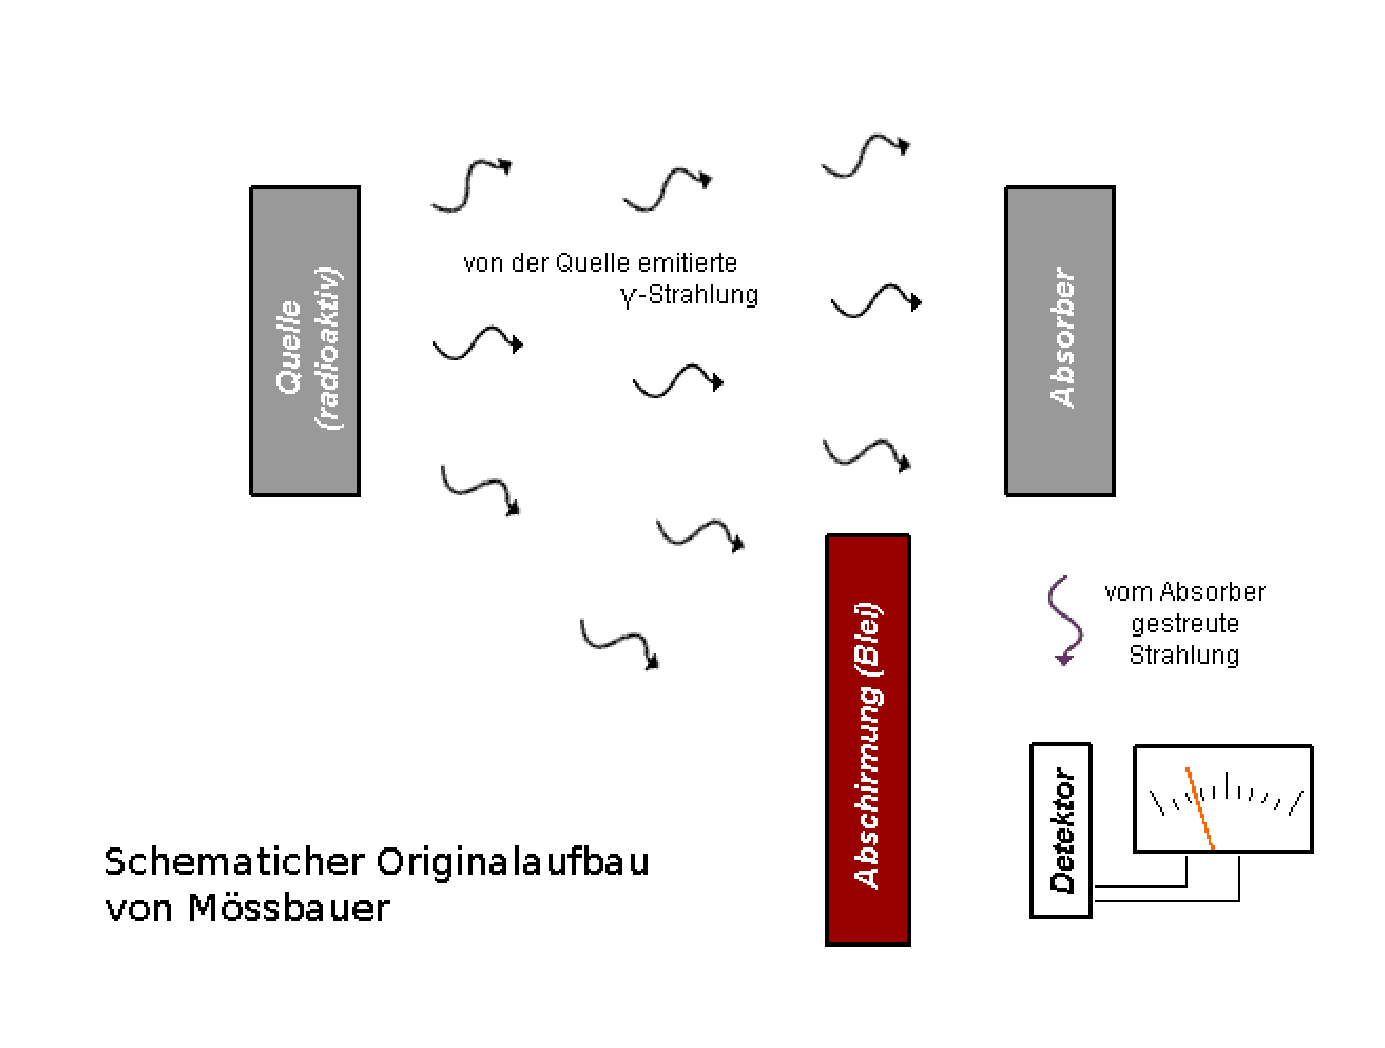
\includegraphics[width=0.9\linewidth]{pictures/moessbauer_original_aufbau.eps}
 \caption{Schematik des Originalaufbaus wie von Mössbauer benutzt}
\end{figure}

in unserem Versuchsaufbau hingegen wird die Transmission des Absorbers hinter diesem detektiert. Hierfür wird ein Szintillationskristall verwendet.

\begin{figure}[H]
 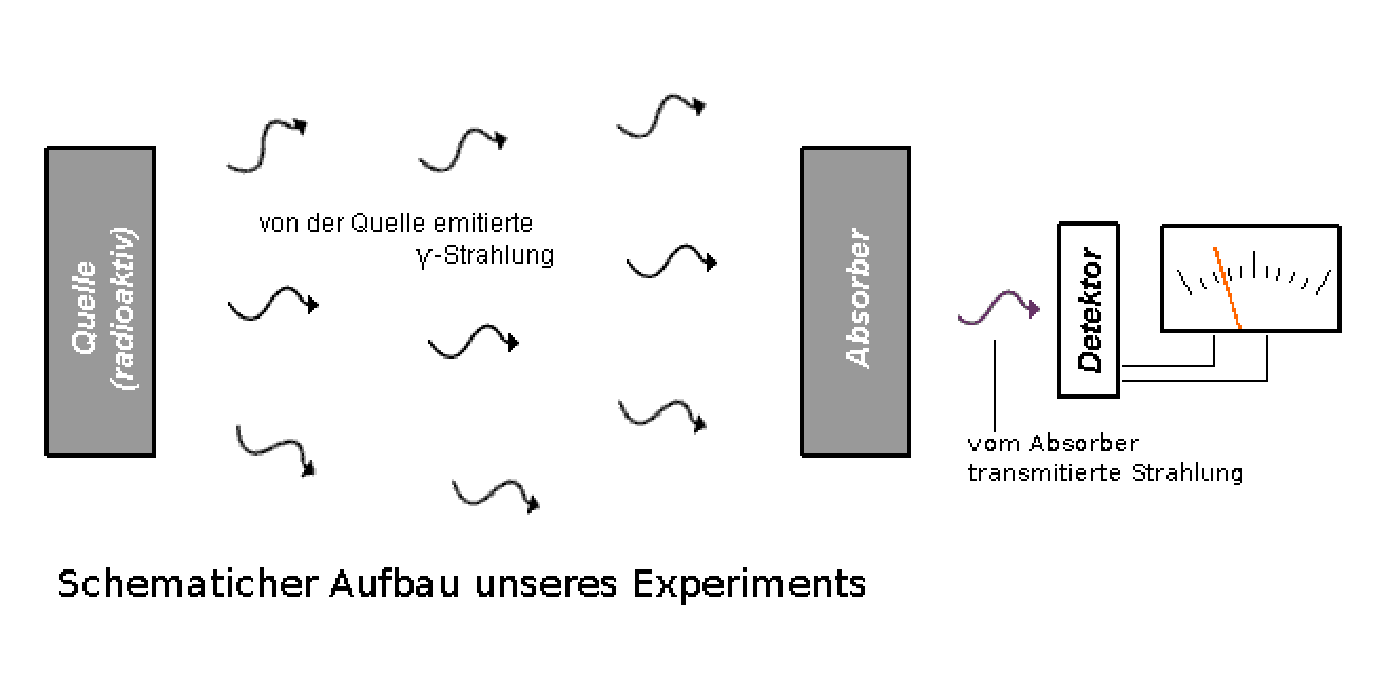
\includegraphics[width=0.9\linewidth]{pictures/unser_aufbau.eps}
 \caption{Energieverschiebung von Emissions- und Absorptionslinie}
\end{figure}

\subsection{Szintillatoren}
beim Durchgang von energiereichen Fotonen oder geladenen Teilchen durch einen Szintillator wird dieser angeregt und gibt diese Anregungsenergie in Form von Licht wieder ab.
man unterscheidet
\begin{itemize}
 \item anorganische Szintillatoren
  mit Aktivatorzentren (Farbzentren) dotierte Kristalle. Ionisierende Strahlung erzeugt freier Elektronen, freie Löcher, oder freie Elektron-Loch-Paare (Exzitzonen).
  Diese wandern bis sie auf ein Aktivatorzentrum treffen, welches in einem angeregten Zustand übergeht und unter Emission von sichtbaren Licht wieder in einen Grundzustand 						zurückfällt. Damit der Szintillationskristall für sein eigenes Licht durchlässig ist muss er ein Einkristall (Monokristall, Kristall einer Atomsorte) sein. Der Donator muss so gewählt sein
  dass er das Leitungs Band des Kristalls derart verformt das an der Fehlstelle Energieniveaus entstehen deren emittierte Fotonen nicht reabsorbiert werden können.
 \item Organische Szintillatoren
  können Kristalle, Flüssigkeiten oder Polymehrere Festkörper sein. Die Szintillation funktioniert durch Anregung von Molekülzuständen in einem primären Fluoreszenzstoff, der 
  dann UV Strahlung emittiert.
\end{itemize}
Wir verwenden einen Szintillationskristall mit Farbstoffdonator.\newline

Das vom Szintillatoren emittierte Licht ist noch zu schwach um direkt gemessen zu werden. Daher verwendet man einen Foto multipler um den Szintillator zu einem Szintillationzähler zu erweitern.

\subsection{Photomultiplier}

ein Photomultiplier ist eine "Photeletktrodenvervielfachungsröhre", also eine Elektronenröhre zur Vervielfältigung von Photonen, also zur Verstärkung sehr schwacher Lichtsignale. Dies wird realisiert durch 
eine Photokathode aus der Photonen durch Photoeffekt Elektronen erzeugen. Diese werden durch eine Spannung, die wie in obiger Skizze zu sehen über eine Spannungsteilerkette gestaffelt an sogenante Dynoden angelegt ist, beschleunigt. 
Bei jedem auftreffen auf solch eine Dynode erzeugt jedes Elektron mehrere Sekundärelektronen (n=3..10) , was eine rasche Vervielfältigung bedeutet. Die Elektronen fliessen schliesslich über die Anode und einen Messwiederstand nach Masse ab. Gemessen wird die Spannung die dabei am Messwiederstand abfällt. \newline

\begin{figure}[H]
 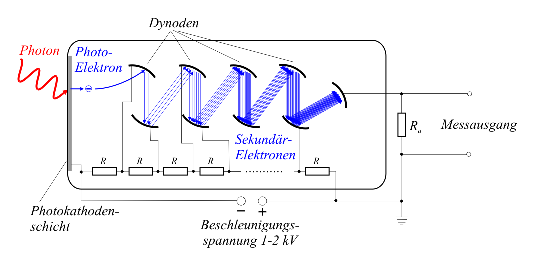
\includegraphics[width=0.9\linewidth]{pictures/photomultiplier_schema.eps}
 \caption{Funktionsprinzip eines Photomultipliers}
\end{figure}

Diese Spannung wird nun elektronisch verarbeitet. Zunächst wird sie vorverstärkt, dann wird sie nach einem konfigurierbarem Verstärker aufgeteilt. Ein Teil geht in einem Fensterdiskriminator der andere in einen so genanntes Linear Gate. 
\section{Durchführung}
\subsection{Energieeichung MCA und Fenstereinstellung}
Um den Multikanalanalysator zum Messen verwenden zu können, muss bekannt sein welche Energie welchem Kanal zugeordnet ist. Hierzu führt man eine Eichung mittels einer bzw. verschiedener
Quellen durch deren bekannte Energien eindeutig identifizierbare Linen im gemessenen Spektrum ergeben. Natürlich hängt die Energie - MCA Kanal Beziehung von der Verstärkereinstellung ab.
Folglich begannen wir damit anhand des Spektrums der $^{57}$Co-Quelle grob zu vermuten wo die zu untersuchende Linie liegt um eine möglichst optimale Auflösung der Linie durch die
Verstärkereinstellung zu erreichen. Hierbei kann man leider nicht an das gewünschte maximum gehen, da der Verstärker sonst übersteuert, was man schön am Oszilloskop beobachten kann.
Als zufriedenstellende Einstellungen gefunden waren konnten wir die Energieeichung mit der Americium-Quelle durchführen. Vor diese Quelle können verschiedene Metallplättchen geschoben
werden um verschiedene Energielinien ($K_\alpha$-Linien) zu erhalten. An die hierbei gemessenen Spektren lies sich jeweils eine Gaußkurve anpassen und schließlich aus den Orten der
einzelenen Gaußkurven und den zugehörigen bekannten Energien ein linearer Zusammenhang zwischen Kanalnummer und Energie herstellen.\\

Nun konnte der $14,4keV$-Peak eindeutig identifiziert werden und wir konnten mit dem SCA das Fenster auf diesen Peak setzen. Das Fenster muss gesetzt werden, da in der eigentlichen
Messung nicht mit dem MCA gemessen wird sonder zwei Counter verwedet werden da diese von der Motorsteuerung aktiviert und deaktiviert werden können. Hierdurch soll sichergestellt werden,
dass nur gemessen wird wenn der Schlitten auch gerade die gewünschte Geschwindigkeit fährt. Für die Einstellung des Fensters, muss das vom Verstärker kommende Signal in den SCA gegeben
werden, dieser entscheidet ob es im Fenster liegt und gibt in diesem fall einen Puls, welcher später vom Counter registriert werden soll, auf seinen Ausgang. Dieses Signal wird verwendet
um ein Gate zu schalten, welches dann wiederum das eigentliche Signal, das vom Verstärker kommt zum MCA durchlässt. Wie man sich denken kann muss dieser Prozess zeitlich abgestimmt
geschehen. Hierfür steht ein Delay zur Verfügung an dem verschiedene Verzögerungen des Signals gewählt werden können. Außerdem bietet der SCA die möglichkeit das Triggersignal verzögert
zu senden. Für die Einstellung werden einfach beide Signale auf dem Oszilloskop betrachtet und über geeignete Verzögerungen Zeitlich in Deckung gebracht.\\

Um sicher zu stellen, dass die von uns gewählte Fenstereinstellung eine Messung möglich machen würde, nahmen wir über jeweils 10 Minuten mittels MCA zwei Kurven auf, eine mit
ruhendem Absorber und eine mit maximaler Absorbergeschwindigkeit. Als wir zwischen diesen beiden Kurven einen Unterschied erkennen konnten waren wir mit der Fenstereinstellung zufrieden.

\subsection{Bestimmung des Untergrunds}
Neben den zwei wesentlichen Peaks im Spektrum der Quelle registriert der Szintillationszähler auch einen Untergrund welcher im wesentlichen durch Comptonstreuung erzeugt wird. Um diesen
Untergrund bestimmen und später von den Messungen abziehen zu können stehen diverse Aluminiumplättchen unterschiedlicher Dicke zur Verfügung. Mit verschiedenen Kombinationen dieser Plättchen nahmen wir
insgesamt 16 Messreihen auf. Wobei wir einen Bereich von $0,2$ bis $12 mm$ Dicke abdeckten. Aus diesen Daten lässt sich später auf die Dicke 0 extrapolieren und somit eine Zählrate für
den Untergrund bestimmen. Mehr dazu in der Auswertung.

\subsection{Messung des Mößbauereffekts}
Nun waren alle Vorbereitungen getroffen um mit der eigenlichen Messung beginnen zu können. Anhand der Zählrate bei unbewegtem Absorber bestimmten wir die benötigte Messdauer pro Geschwindigkeit,
welche den Fehler unter 1\% bringen würde. Während wir Messreihen zu verschiedenen Geschwindigkeiten aufnahmen, haben wir die erhaltenen Daten direkt in eine Grafik geplottet um abschätzen
zu können wann eine ausreichene Punktdichte erreicht ist. Da die Labviewsoftware leider des öfteren nicht so wollte wie wir ging das Messen relativ lange, oft hatten wir Messreihen für die ganze
Nacht geplant um dann am nächtsten Morgen festzustellen, dass nur zwei Stunden gemessen wurde. Schlussendlich haben wir es aber geschafft in den zwei Wochen die beiden Absorber (1-Linien und 6-Linien)
mit ausreichen vielen Geschwindigkeiten durchzufahren um den Kurvenverlauf durch viele Punkte abzudecken. Es stellte sich heraus, dass es sehr wichtig ist die Spannung am Szintillationszähler konstant
zu halten. Hier haben schon geringe Abweichungen von der Sollspannung die Konsistenz der Messdaten zerstört. Eine Änderung der eingestellten Spannung trat allerdings nur auf wenn das Netzteil
abgestürzt war und die Spannung wieder neu gesetzt werden musste. Ein Absturz des Netzteils war zu erreichen indem man die Motorsteuerung aus und wieder an schaltete, was meistens nötig war
wenn die Labviewsoftware sich mal wieder aufgehängt hatte. Abgesehen von diesen kleinen Problemen verlief die Messung sonst Problemlos, sogar das Schalten des Getiebes erwies sich nach ein bisschen
Übung als sehr einfach.
\section{Auswertung}
\subsection{Energieeichung}

Um den Kanälen des MCA einen Energiewert zuordnen zu können führten wir zunächst eine Energieeichung durch. Dazu hatten wir folgende fünf Proben mit $K\alpha$ Übergängen
bekannter Energien zur Verfügung:
\begin{itemize}
 \item Rubidium bei\hspace{30pt}13.37 keV
 \item Molibdän bei\hspace{30pt}17.44 keV
 \item Silber	bei\hspace{30pt}22.10 keV
 \item Terbium  bei\hspace{30pt}44.23 keV
 \item Barium   bei\hspace{30pt}32.06 keV
\end{itemize}

wir nahmen also deren Spektren auf, führten Gaussfits an die oben genannten Linien durch und erhielten so fünf Kanalwerte bekannter Energien. An diese fitteten 
wir eine Gerade (der lineare Zusammenhang zwischen Kanal und Energie ist nirgends explizit erwähnt, aber natürlich dringend notwendig) um folgende Parameter
zu erhalten, hierbei ist $C$ der Kanal, $E$ die Energie und $a,b$ die Fitparameter.
\begin{align*}
  C = a \cdot E + b \hspace{30pt} \textnormal{mit }a = 100.52 \pm 0.04\textnormal{ und }b =  -62.42 \pm 1.285
\end{align*}
wobai für den Fehler die Gaußsche Fehlerfortpflanzung anzuwenden ist:
\begin{align*}
  s_C = \sqrt{\frac{\partial{c}}{\partial{a}}^2 s_a^2 + \frac{\partial{C}}{\partial{b}}^2 s_b^2 } = \sqrt{E^2 s_a^2 + s_b^2}
\end{align*}

Dieses Ergebniss benutzten wir um den 14.4 keV Peak unseres Eisens zu identifizieren. Als Erwarteten Kanal erhält man also:
\begin{align*}
  C_{14.4keV} = 1385,07 \pm 1,27
\end{align*}

Wie in Abbildung \ref{spek} zu sehen entspricht der Schwerpunkt des Gaußfits $\mu=1386.24\pm0.15$ in den Fehlergrenzen dem erwarteten Kanal. Wir wissen also nun mit Gewissheit
welcher Peak der für uns interessante ist.

\begin{figure}[H]
 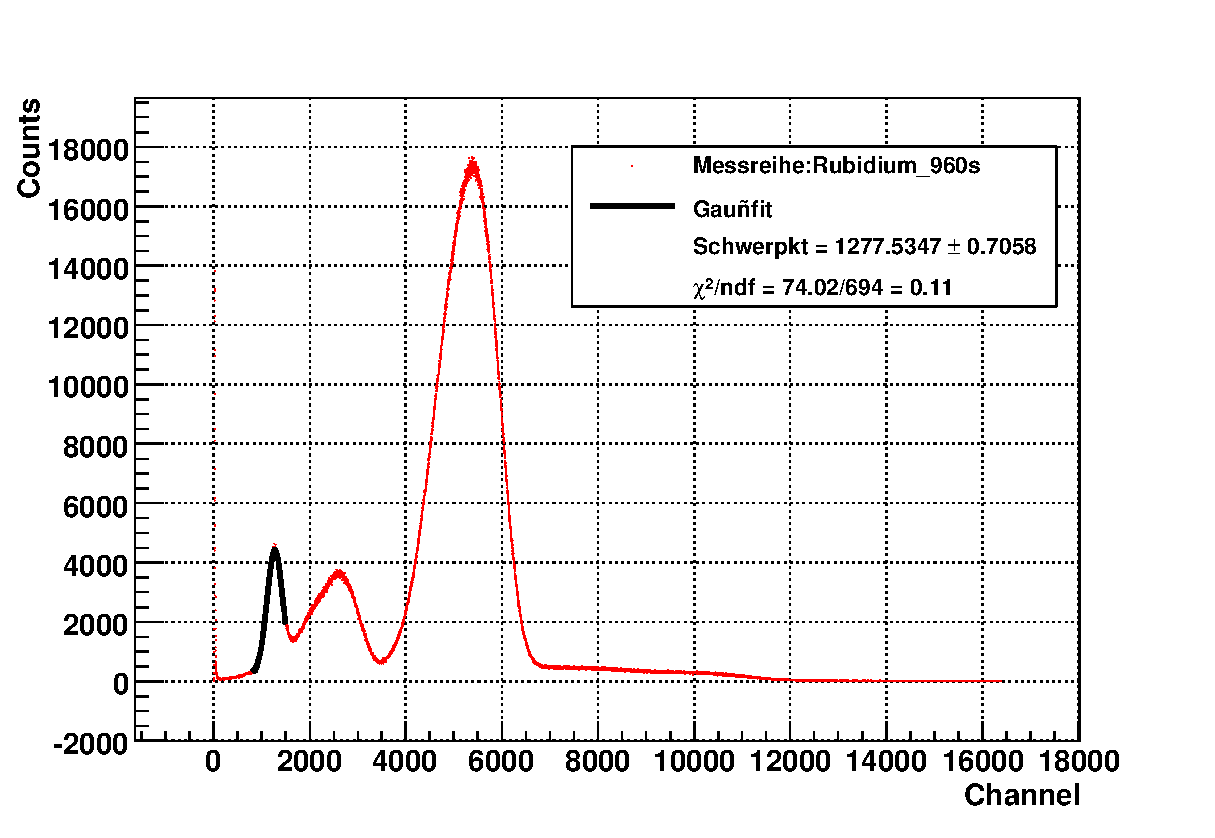
\includegraphics[width=0.9\linewidth]{pictures/eichung_rubidium.eps}
 \caption{Gaußfit an Rubbidium}
\end{figure}
\begin{figure}[H]
 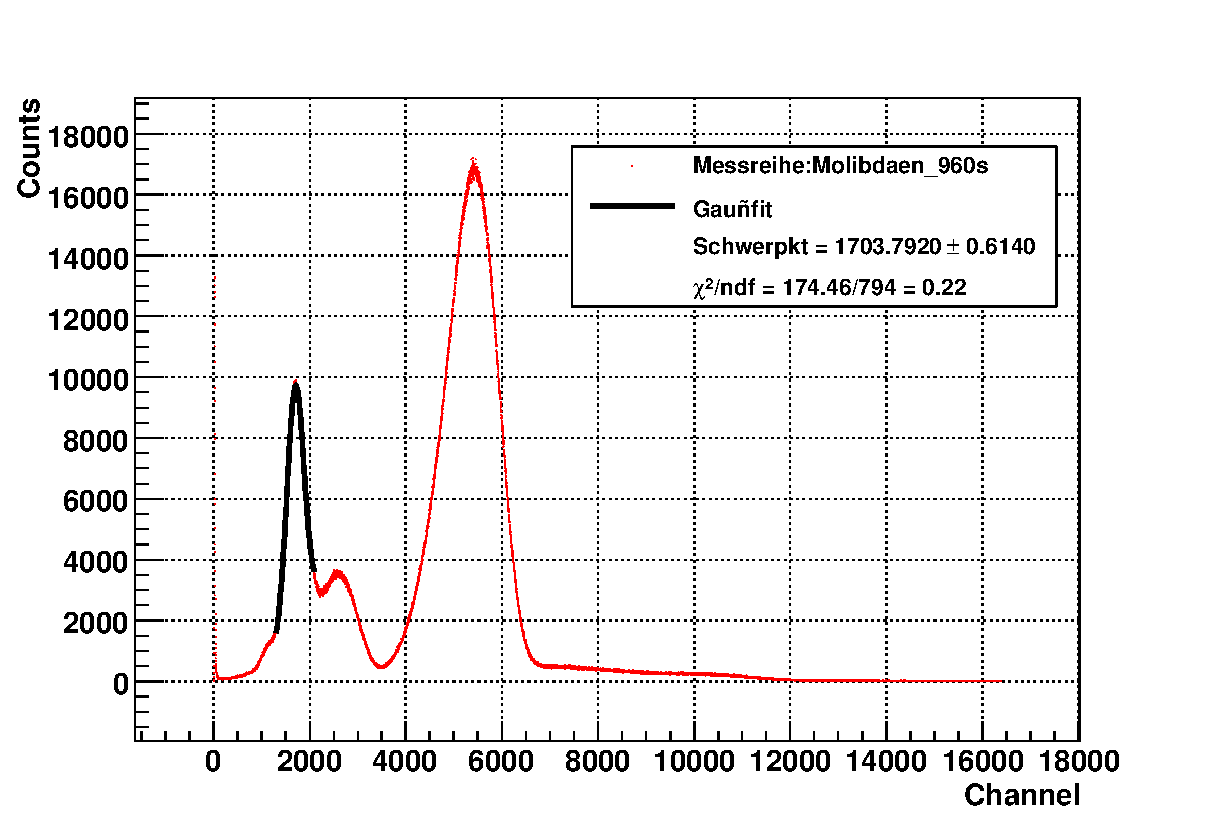
\includegraphics[width=0.9\linewidth]{pictures/eichung_molibdaen.eps}
 \caption{Gaußfit an Molibdän}
\end{figure}
\begin{figure}[H]
 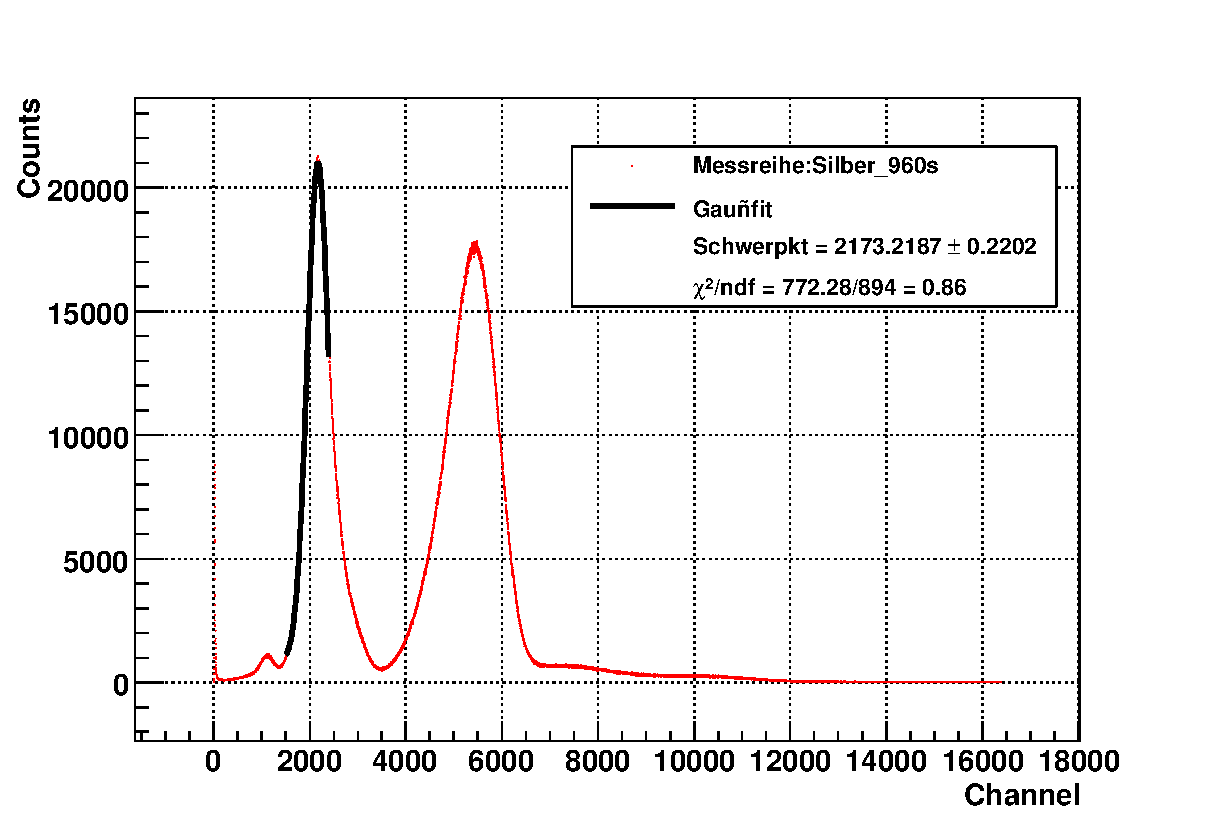
\includegraphics[width=0.9\linewidth]{pictures/eichung_silber.eps}
 \caption{Gaußfit an Silber}
\end{figure}
\begin{figure}[H]
 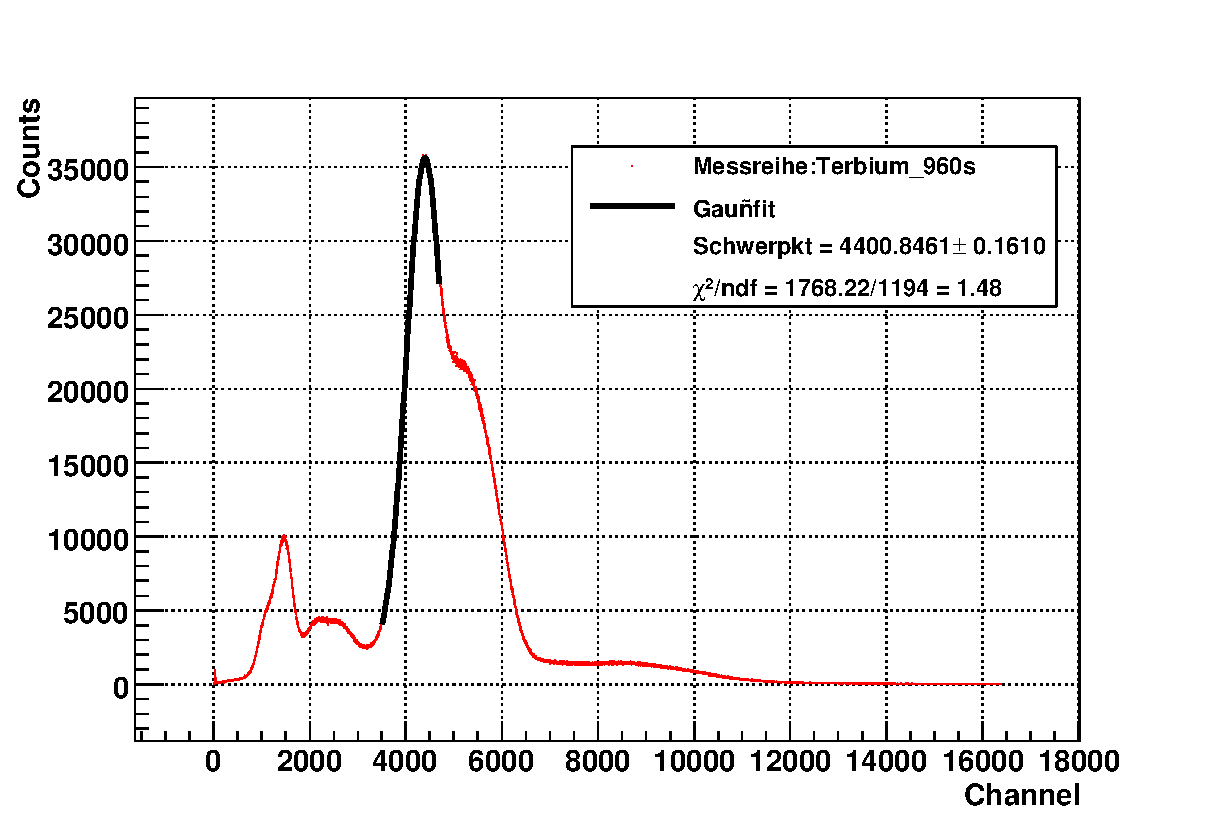
\includegraphics[width=0.9\linewidth]{pictures/eichung_terbium.eps}
 \caption{Gaußfit an Terbium}
\end{figure}
\begin{figure}[H]
 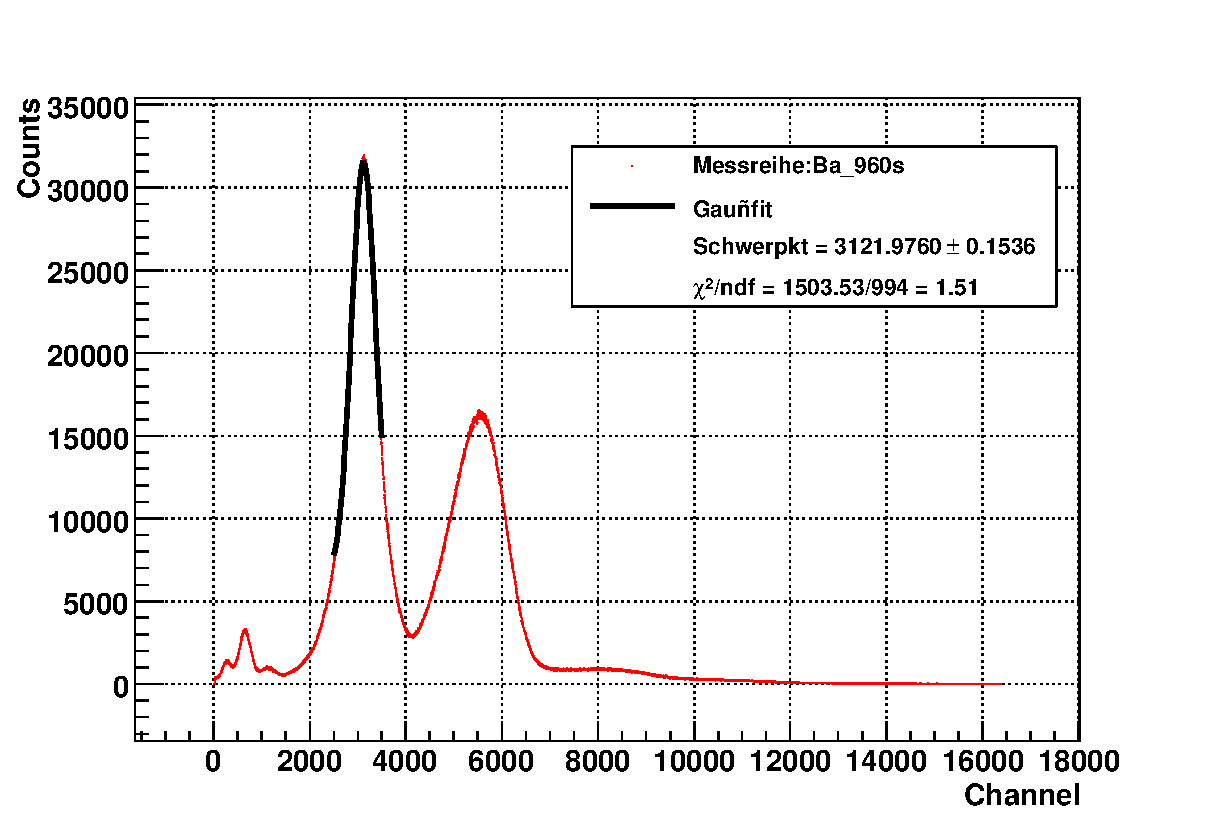
\includegraphics[width=0.9\linewidth]{pictures/eichung_barium.eps}
 \caption{Gaußfit an Barium}
\end{figure}
\begin{figure}[H]
 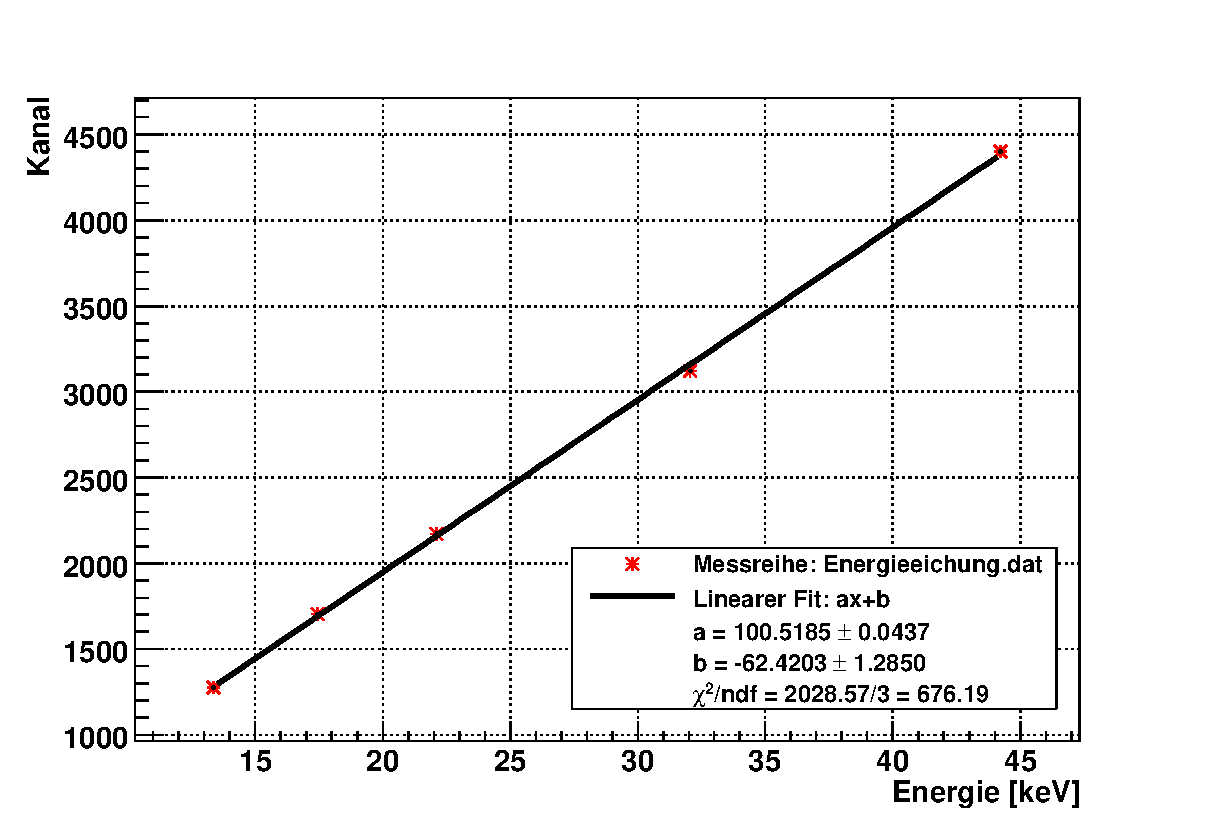
\includegraphics[width=0.9\linewidth]{pictures/eichung_linear.eps}
 \caption{linearer Fit an die bekannten Energien}
\end{figure}
\begin{figure}[H]
 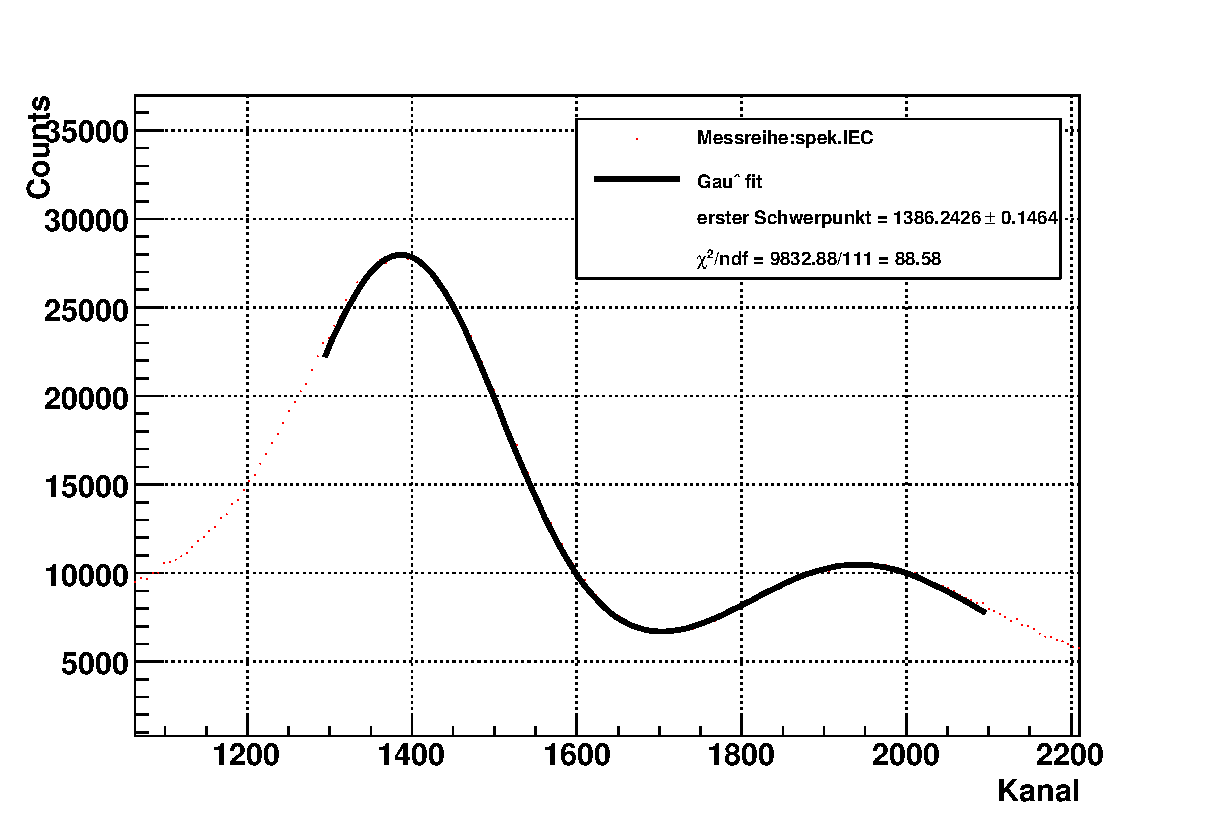
\includegraphics[width=0.9\linewidth]{pictures/eichung_spek.eps}
 \caption{Gaußfit an 14,4keV Linie von Eisen}
\label{spek}
\end{figure}

\subsection{Untergrund}
Da bei dem Zerfall von $^{57}Co$ nach $^{57}Fe$ im Wesentlichen zwei Energien ($14,4 keV$ und $122 keV$ bzw. $136 keV$
\footnote{Der $136 keV$-Übergang ist relativ selten und liegt im Vergleich zu dem 14,4 keV sehr nah an dem $122 keV$-Übergang. Aus diesem Grund kann in guter
Näherung von nur zwei verschiedenen Energien ausgegangen werden.}). Bei der Abschirmung durch Aluminium erwartet man also bei zunehmender Plättchendicke
unterschiedlich starke Abschwächung der beiden Energien. Fittet man also eine Überlagerung von zwei Expotentialfunktionen an den gemessenen Verlauf, kann auf
die Abschwächung der einzelnen Energien zurückgeschlossen werden. Wir erhalten somit einen Wert für den Untergrund in unserem $14,4 keV$ Fenster.\\

Die Dicke des Aluminiumabsorbers haben wir jeweils mit der Mikrometerschraube gemessen und einen Fehler von $0,01 mm$ auf diese angenommen. Da die Mikrometerschraube leider wohl schon mal mit Gewalt in Berührung kam, hat diese einen Offset den man nicht übersehen sollte.
Der Fehler auf die Zählrate $R = \frac{N}{t}$ ergibt sich zu:
\begin{align}
 s_R = R \sqrt{\left(\frac{s_t}{t}\right)^2 + \frac{1}{\sqrt{N}}}
\end{align}

Durch die relativ langen Messdauern (teilweise über Nacht gemessen) wird dieser Fehler allerdings so klein, dass ROOT keinen Fit mehr hinbekommt.
Möglicherweise liegt hier ein systematischer Fehler vor der mit den Plättchen zusammenhängt oder von den ``Witterungsbedingungen'' abhängig ist.
Gefittet wurde also mit der \textit{W} Option\footnote{\textit{W} - Set all weights to 1; ignore error bars}. Der Fit berücksichtigt also leider nicht, dass die Punkte die über Nacht gemessen wurden eigentlich einen kleineren Fehler haben als die Anderen. Aus dem Fit ergab sich folgender Zusammenhang für Dicke und Abschwächung der höheren Energie:
\begin{align*}
 f_2 (d) = (50,38 \pm 0,78) \cdot exp (-0,0413 \pm 0,0027) \frac{Counts}{s}
\end{align*}
 und somit eine Zählrate für den Untergrund bei Dicke 0 in unserm Fenster von:
\begin{align*}
 R_{Untergrund} = (50,38 \pm 0,78) \frac{Counts}{s} 
\end{align*}
Diese Rate wurde in allen folgenden Messungen abgezogen.
       

\begin{figure}[H]
 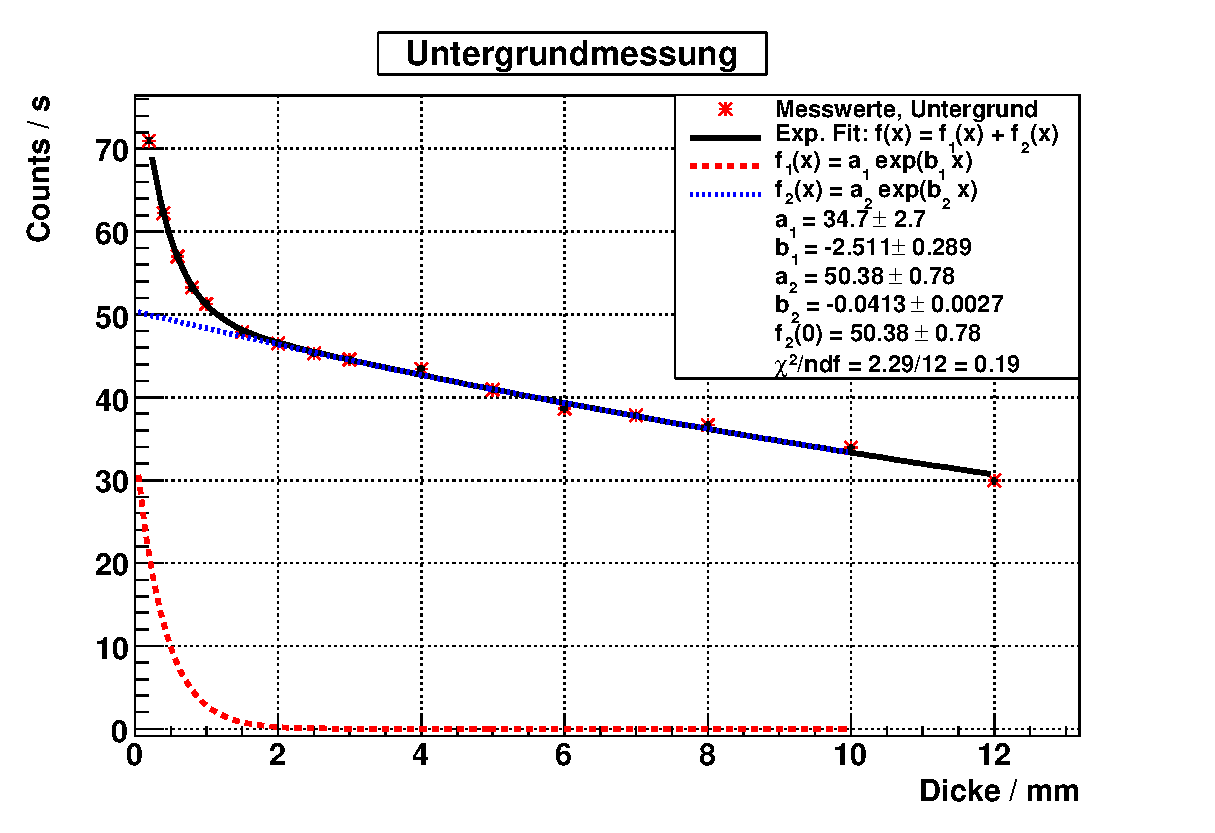
\includegraphics[width=0.9\linewidth]{pictures/untergrund.eps}
 \caption{Untergrund extrapolation auf Absorberdicke 0}
\end{figure}

\subsection{1-Linien-Absorber (Edelstahl)}

\subsection{6-Linien-Absorber (Eisen)}

Beim 6-Linien-Absorber sollen die Isomerievershiebung, das kernmagnetisch Moment $\mu_a$ des angeregten Zustandes und die magnetische Feldstärke $B$
am Kernort bestimmt werden. Leider schafften wir mit unseren Daten die für 2 wöchige Gruppen optional gestellte Aufgabe der Bestimmung des
Debeye-Waller-Faktors und der Lebensdauer des angeregten Zustands nicht. Daher sind in Abbildung \refname{eisen} Die Messdaten sowie eine schsfache
Überlagerung eines Lorentzfits zu sehen. Zunächst ordnen wir die Peaks aber nach ihren quantenmechanischen Übergängen. 
\begin{figure}[H]
 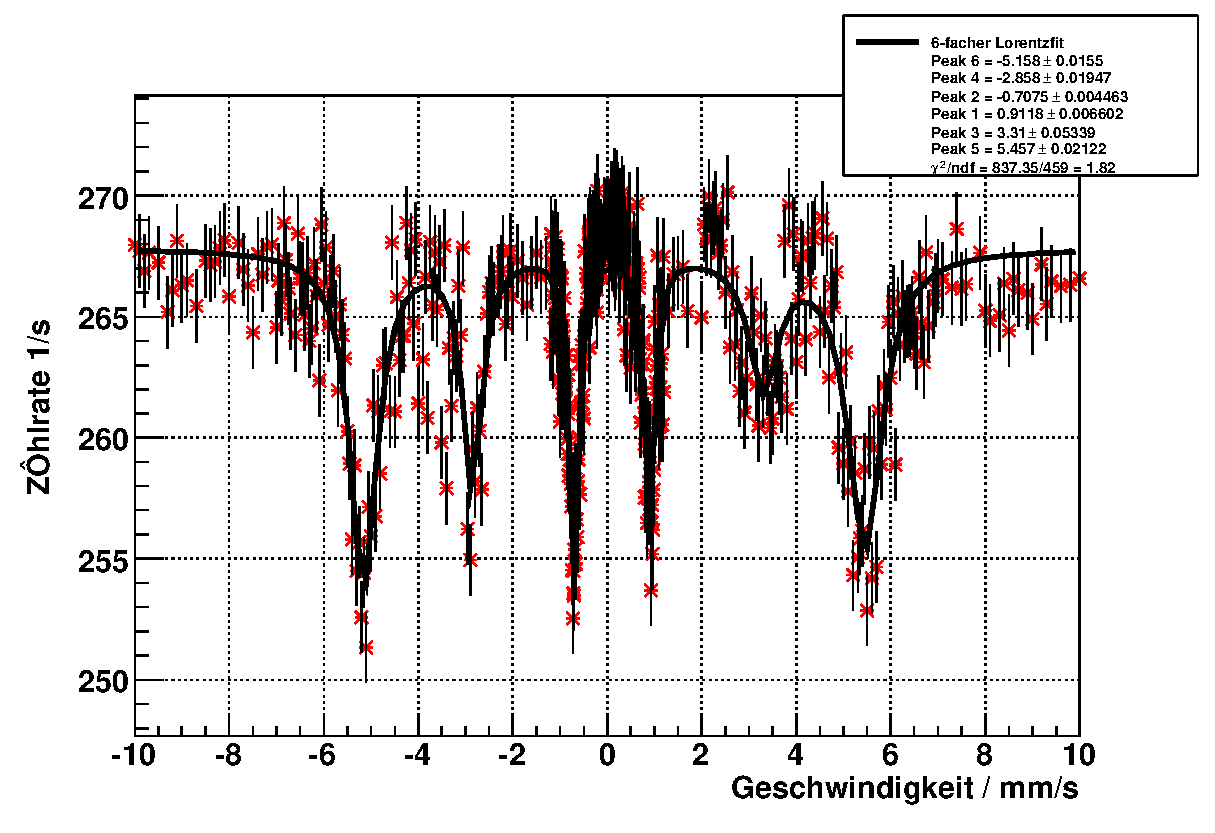
\includegraphics[width=0.9\linewidth]{pictures/eisen.eps}
 \caption{sechfacher Lorentzfit an Messdaten aus Eisenmessung}
\end{figure}

Die Energien $E_i$ der Absorptionslinien lassen sich nach Gleichung \ref{hfs} berechnen zu:
\begin{align*}
 E_i = E_{iso} - E_{hfs}^i \hspace{5pt} \textnormal{    mit } E_{hfs}^i = \left( \frac{\mu_a m_a^i}{I_a} - \frac{\mu_g m_g^i}{I_g} \right) B
\end{align*}
oder, umformuliert auf die zu den Energien gehörigen Geschwidigkeiten des Messschlittens:
\begin{align*}
 v_i = v_{iso} - v_{hfs}^i \hspace{5pt} \textnormal{    mit } v_{hfs}^i = \frac{c}{E_0} E_{hfs}^i = \frac{c}{E_0} \left( \frac{\mu_a m_a^i}{I_a} - \frac{\mu_g m_g^i}{I_g} \right) B
\end{align*}
\label{geschw}
berücksichtigt man nun die Auswahlregel für Dipolstrahlung ($\Delta m = 0, \pm 1$) so erhält man 6 mögliche Übergänge, einen für jeden Peak. Berechnet man 
nun mit obiger Formel $v_{hfs}^i$, so fällt auf das sich jeweils 2 Geschwindigkeiten immer nur um das Vorzeichen Unterscheiden.
Desweiteren sind in folgender Tabelle die aus dem Fit gewonnenen Geschwindigkeiten der Peaks sowie deren daraus resultierender Energie mit relativen Fehlern
eingetragen:
\begin{center}
\begin{tabular}{|l|llllll|}
\hline
Peak i & $\mu_a^i$ & $\mu_g^i$ & $v_{hfs}^i$ & $v_{mes}^i/\frac{mm}{s}$ & $E_{mes}^i/10^{-7} eV$ & \% Fehler\\
\hline
1 & $+\frac{3}{2}$ & $+\frac{1}{2}$ & $v_1$ & -5.158 & -2.48 & 0.72\\
2 & $+\frac{1}{2}$ & $+\frac{1}{2}$ & $v_2$ & -2.858 & -1.37 & 0.63\\
3 & $-\frac{1}{2}$ & $+\frac{1}{2}$ & $v_3$ & -0.7075 & -0.34 & 1.61\\
4 & $+\frac{1}{2}$ & $-\frac{1}{2}$ & $-v_3$ & 0.9118 & -0.44 & 0.68\\
5 & $-\frac{1}{2}$ & $-\frac{1}{2}$ & $-v_2$ & 3.31 & 1.59 & 0.39\\
6 & $-\frac{3}{2}$ & $-\frac{1}{2}$ & $-v_1$ & 5.457 & 2.62 & 0.3\\
\hline
\end{tabular}
\label{eisen_tab1}
\end{center}
\subsubsection{Isomerieverschiebung}
Aus Gleichung \ref{geschw} und $v_{mes}^i = v_{hfs}^i + v_{iso}$ folgt sofort die Formel zur bestimmung der Isomerieverschiebung. Die zuordnung 
der Peaks folgt aus obiger Tabelle.
\begin{align*}
 v_{iso} = \frac{v_{mes}^1+v_{mes}^6}{2} =\frac{v_{mes}^2+v_{mes}^5}{2} =\frac{v_{mes}^3+v_{mes}^4}{2}
\end{align*}
Wir erhielten als Ergenisse: \\
\newline
\begin{center}
\begin{tabular}{|l|lll|}
\hline
Peaks & $v_{iso}/\frac{mm}{s}$ & $E_{iso}/10^{-9}eV$ & \% Fehler\\
\hline
1 und 6& $-0.1021 \pm 0.004$ & $-4.91 \pm 0.19$ & 3.9\\
2 und 5& $-0.2262 \pm 0.028$ & $-10.8 \pm 1.4$ & 12.56\\
1 und 6& $-0.1497 \pm 0.013$ & $-7.195 \pm 0.63$ & 8.78\\
\hline
\end{tabular}
\label{eisen_tabiso}
\end{center}

Bildet man daraus das gewichtete Mittel, so erhält man:
\begin{align*}
 v_{iso} = (-0.1083\pm 0.0038)\frac{mm}{s} \\
 E_{iso} = (-5.205 \pm 0.18)10^{-9} eV
\end{align*}

\section{Zusammenfassung}

\section{Zusatz: Geschwindigkeitsmessung oder die entdeckung der Langsamkeit}
Nach Aussagen des Assistenten stellte sich bei diesem Versuchsaufbau schon seit längerem die Frage wie groß der Fehler der Geschindigkeit des Schlittens also des Absorbers ist. Somit haben wir uns ein paar Gedanken gemacht wie man denn die Geschwindikeit des Schlittens Messen kann. Eine Zeitmessung über lange Strecken macht keinen Sinn, da die Konstanz der Geschindigkeit untersucht werden soll. Wir hatten die Idee den Sensor einer optischen Maus zu verwenden: 800 dpi, sollten eine ausreichende Genauigkeit bringen.

Gängige Maussensoren haben zwei mögliche Ausgänge: Ein serieller Ausgang und eine ``Quadratur Ausgang'' also 2 Pins für jede Achse, wobei die Zustände im Ring je nach Bewegungsrichtung linksrum oder rechtsrum aufeinander folgen.

Wir entschienden uns mit der Intention die kleinstmöglichen Inkremente zu erhalten für den letzeren Anschluss und nahmen einen Microcontroller für die Auswertung der Bewegung. Anfangs war das ein Microchip PIC18F4550, da dieser jedoch Probleme machte stiegen wir auf einen Atmel ATMega32 um. Leider mussten wir feststellen als wir die ersten Geschwindigkeitshistogramme betrachteten, dass ein Fehler vorlag. Es stellte sich heraus das der 16MHz Takt des Microcontrollers nicht ausreichte um alle Zustandsänderungen des Maussensors zu erfassen. Bei schnellen Bewegungen kam der Chip nicht nach einem Interrupt nicht mehr in den normalen Programmablauf da schon der nächste Interrupt ausgelöst war.


Also musste doch die 1te Anschlussmethode herhalten, diesmal aber ohne Microcontroller und stattdessen direkt am PC angeschlossen.

Nachdem das Programm geschrieben und die ersten Messungen gemacht waren wurde schnell klar das wir einen noch falscheren Weg eingeschlagen hatten, denn nun verpassten wir zwar keinenWeginkrement mehr, allerdings 
lag nun die Genauigkeit der Zeitmessung an der Prozessorauslastung des Rechners. Da dies noch unzulänglicher war überdachten wir unseren ersten Ansatz, und implementiereten eine Version in der über eine einstellbare Anzahl von Weginkrementen gemittelt wird.
Dies erwies sich als des Rätsels Lösung. Wir hatten zwar die Anzahl der Messungen deutlich reduziert, dafür war die Aufgabe die der Microcontroller nun wärend eines Interrupts zu tun hatte (zählen) nicht mehr rechenintensiv, wesshalb es nun nicht mehr zu ``doppelten Interrupts'' kam.
Desweiteren hatten wir den Fehler unserer Messung nun deutlich reduziert. Leider hatten wir Hard- und Software erst am letzten Tag unseres Praktikums bugfrei, wesshalb wir nicht mehr viele Datenreihen aufnehmen konnten. Die Aufgenommenen lieferten allerdings wie wir finden ein 
Ergebniss, das durchaus Verbesserungsmöglichkeiten aufzeigt.

\end{document}
